% Options for packages loaded elsewhere
\PassOptionsToPackage{unicode,linktoc=all}{hyperref}
\PassOptionsToPackage{hyphens}{url}
\PassOptionsToPackage{dvipsnames,svgnames,x11names}{xcolor}
%
\documentclass[
  a4paper,
]{article}
\usepackage{amsmath,amssymb}
\usepackage{iftex}
\ifPDFTeX
  \usepackage[T1]{fontenc}
  \usepackage[utf8]{inputenc}
  \usepackage{textcomp} % provide euro and other symbols
\else % if luatex or xetex
  \usepackage{unicode-math} % this also loads fontspec
  \defaultfontfeatures{Scale=MatchLowercase}
  \defaultfontfeatures[\rmfamily]{Ligatures=TeX,Scale=1}
\fi
\usepackage{lmodern}
\ifPDFTeX\else
  % xetex/luatex font selection
\fi
% Use upquote if available, for straight quotes in verbatim environments
\IfFileExists{upquote.sty}{\usepackage{upquote}}{}
\IfFileExists{microtype.sty}{% use microtype if available
  \usepackage[]{microtype}
  \UseMicrotypeSet[protrusion]{basicmath} % disable protrusion for tt fonts
}{}
\makeatletter
\@ifundefined{KOMAClassName}{% if non-KOMA class
  \IfFileExists{parskip.sty}{%
    \usepackage{parskip}
  }{% else
    \setlength{\parindent}{0pt}
    \setlength{\parskip}{6pt plus 2pt minus 1pt}}
}{% if KOMA class
  \KOMAoptions{parskip=half}}
\makeatother
\usepackage{xcolor}
\usepackage[margin=25mm]{geometry}
\usepackage{longtable,booktabs,array}
\usepackage{calc} % for calculating minipage widths
% Correct order of tables after \paragraph or \subparagraph
\usepackage{etoolbox}
\makeatletter
\patchcmd\longtable{\par}{\if@noskipsec\mbox{}\fi\par}{}{}
\makeatother
% Allow footnotes in longtable head/foot
\IfFileExists{footnotehyper.sty}{\usepackage{footnotehyper}}{\usepackage{footnote}}
\makesavenoteenv{longtable}
\usepackage{graphicx}
\makeatletter
\def\maxwidth{\ifdim\Gin@nat@width>\linewidth\linewidth\else\Gin@nat@width\fi}
\def\maxheight{\ifdim\Gin@nat@height>\textheight\textheight\else\Gin@nat@height\fi}
\makeatother
% Scale images if necessary, so that they will not overflow the page
% margins by default, and it is still possible to overwrite the defaults
% using explicit options in \includegraphics[width, height, ...]{}
\setkeys{Gin}{width=\maxwidth,height=\maxheight,keepaspectratio}
% Set default figure placement to htbp
\makeatletter
\def\fps@figure{htbp}
\makeatother
\usepackage{svg}
\setlength{\emergencystretch}{3em} % prevent overfull lines
\providecommand{\tightlist}{%
  \setlength{\itemsep}{0pt}\setlength{\parskip}{0pt}}
\setcounter{secnumdepth}{-\maxdimen} % remove section numbering
% definitions for citeproc citations
\NewDocumentCommand\citeproctext{}{}
\NewDocumentCommand\citeproc{mm}{%
  \begingroup\def\citeproctext{#2}\cite{#1}\endgroup}
\makeatletter
 % allow citations to break across lines
 \let\@cite@ofmt\@firstofone
 % avoid brackets around text for \cite:
 \def\@biblabel#1{}
 \def\@cite#1#2{{#1\if@tempswa , #2\fi}}
\makeatother
\newlength{\cslhangindent}
\setlength{\cslhangindent}{1.5em}
\newlength{\csllabelwidth}
\setlength{\csllabelwidth}{3em}
\newenvironment{CSLReferences}[2] % #1 hanging-indent, #2 entry-spacing
 {\begin{list}{}{%
  \setlength{\itemindent}{0pt}
  \setlength{\leftmargin}{0pt}
  \setlength{\parsep}{0pt}
  % turn on hanging indent if param 1 is 1
  \ifodd #1
   \setlength{\leftmargin}{\cslhangindent}
   \setlength{\itemindent}{-1\cslhangindent}
  \fi
  % set entry spacing
  \setlength{\itemsep}{#2\baselineskip}}}
 {\end{list}}
\usepackage{calc}
\newcommand{\CSLBlock}[1]{\hfill\break#1\hfill\break}
\newcommand{\CSLLeftMargin}[1]{\parbox[t]{\csllabelwidth}{\strut#1\strut}}
\newcommand{\CSLRightInline}[1]{\parbox[t]{\linewidth - \csllabelwidth}{\strut#1\strut}}
\newcommand{\CSLIndent}[1]{\hspace{\cslhangindent}#1}
\ifLuaTeX
\usepackage[bidi=basic]{babel}
\else
\usepackage[bidi=default]{babel}
\fi
\babelprovide[main,import]{british}
% get rid of language-specific shorthands (see #6817):
\let\LanguageShortHands\languageshorthands
\def\languageshorthands#1{}
% $HOME/.pandoc/defaults/latex-header-includes.tex
% Common header includes for both lualatex and xelatex engines.
%
% Preliminaries
%
% \PassOptionsToPackage{rgb,dvipsnames,svgnames}{xcolor}
% \PassOptionsToPackage{main=british}{babel}
\PassOptionsToPackage{english}{selnolig}
\AtBeginEnvironment{quote}{\small}
\AtBeginEnvironment{quotation}{\small}
\AtBeginEnvironment{longtable}{\centering}
%
% Packages that are useful to include
%
\usepackage{graphicx}
\usepackage{subcaption}
\usepackage[inkscapeversion=auto]{svg}
\usepackage{nowidow}
\usepackage{etoolbox}
\usepackage{fontsize}
\usepackage{newunicodechar}
\usepackage{pdflscape}
\usepackage{fnpct}
\usepackage{parskip}
  \setlength{\parindent}{0pt}
\usepackage[style=american]{csquotes}
% \usepackage{setspace} Use the <fontname-plus.tex> files for setspace
%
\usepackage{hyperref} % cleveref must come AFTER hyperref
\usepackage[capitalize,noabbrev]{cleveref} % Must come after hyperref
\let\longdivision\relax
\usepackage{longdivision}
\newcommand{\dd}{\ensuremath{mathrm d}}
%
% Assume that amsmath is already loaded via \usepackage{amsmath}
% in the standard LaTeX template foe Pandoc
% 
\DeclareMathOperator{\sech}{sech}
\DeclareMathOperator{\csch}{csch}
\DeclareMathOperator{\arcsec}{arcsec}
\DeclareMathOperator{\arccot}{arccot}
\DeclareMathOperator{\arccsc}{arccsc}
\DeclareMathOperator{\arccosh}{arccosh}
\DeclareMathOperator{\arcsinh}{arcsinh}
\DeclareMathOperator{\arctanh}{arctanh}
\DeclareMathOperator{\arcsech}{arcsech}
\DeclareMathOperator{\arccsch}{arccsch}
\DeclareMathOperator{\arccoth}{arccoth} 
% noto-plus.tex
% Font-setting header file for use with Pandoc Markdown
% to generate PDF via LuaLaTeX.
% The main font is Noto Serif.
% Other main fonts are also available in appropriately named file.
\usepackage{fontspec}
\usepackage{setspace}
\setstretch{1.3}
%
\defaultfontfeatures{Ligatures=TeX,Scale=MatchLowercase,Renderer=Node} % at the start always
%
% For English
% See also https://tex.stackexchange.com/questions/574047/lualatex-amsthm-polyglossia-charissil-error
% We use Node as Renderer for the Latin Font and Greek Font and HarfBuzz as renderer ofr Indic fonts.
%
\babelfont{rm}[Script=Latin,Scale=1]{NotoSerif}% Config is at $HOME/texmf/tex/latex/NotoSerif.fontspec
\babelfont{sf}[Script=Latin]{SourceSansPro}% Config is at $HOME/texmf/tex/latex/SourceSansPro.fontspec
\babelfont{tt}[Script=Latin]{FiraMono}% Config is at $HOME/texmf/tex/latex/FiraMono.fontspec
%
% Sanskrit, Tamil, and Greek fonts
%
\babelprovide[import, onchar=ids fonts]{sanskrit}
\babelprovide[import, onchar=ids fonts]{tamil}
\babelprovide[import, onchar=ids fonts]{greek}
%
\babelfont[sanskrit]{rm}[Scale=1.1,Renderer=HarfBuzz,Script=Devanagari]{NotoSerifDevanagari}
\babelfont[sanskrit]{sf}[Scale=1.1,Renderer=HarfBuzz,Script=Devanagari]{NotoSansDevanagari}
\babelfont[tamil]{rm}[Renderer=HarfBuzz,Script=Tamil]{NotoSerifTamil}
\babelfont[tamil]{sf}[Renderer=HarfBuzz,Script=Tamil]{NotoSansTamil}
\babelfont[greek]{rm}[Script=Greek]{GentiumBookPlus}
%
% Math font
%
\usepackage{unicode-math} % seems not to hurt % fallabck
\setmathfont[bold-style=TeX]{STIX Two Math}
\usepackage{amsmath}
\usepackage{esdiff} % for derivative symbols
% \renewcommand{\mathbf}{\symbf}
%
%
% Other fonts
%
\newfontfamily{\emojifont}{Symbola}
%

\usepackage{titling}
\usepackage{fancyhdr}
    \pagestyle{fancy}
    \fancyhead{}
    \fancyfoot{}
    \renewcommand{\headrulewidth}{0.2pt}
    \renewcommand{\footrulewidth}{0.2pt}
    \fancyhead[LO,RE]{\scshape\thetitle}
    \fancyfoot[CO,CE]{\footnotesize Copyright © 2006\textendash\the\year, R (Chandra) Chandrasekhar}
    \fancyfoot[RE,RO]{\thepage}
%
\usepackage{newunicodechar}
\newunicodechar{√}{\textsf{√}}
\usepackage {caption}
    \captionsetup{font={sf,stretch=1.4}}
\ifLuaTeX
  \usepackage{selnolig}  % disable illegal ligatures
\fi
\IfFileExists{bookmark.sty}{\usepackage{bookmark}}{\usepackage{hyperref}}
\IfFileExists{xurl.sty}{\usepackage{xurl}}{} % add URL line breaks if available
\urlstyle{sf}
\hypersetup{
  pdftitle={Expressions, Equations, and Formulae},
  pdfauthor={R (Chandra) Chandrasekhar},
  pdflang={en-GB},
  colorlinks=true,
  linkcolor={DarkGreen},
  filecolor={Purple},
  citecolor={Teal},
  urlcolor={Maroon},
  pdfcreator={LaTeX via pandoc}}

\title{Expressions, Equations, and Formulae}
\author{R (Chandra) Chandrasekhar}
\date{2025-02-10 | 2025-02-15}

\begin{document}
\maketitle

\thispagestyle{empty}


\subsection{An unforeseen challenge}\label{an-unforeseen-challenge}

My dear friend, Solus ``Sol'' Simkin, casually asked me one summer day
if I would write a blog demystifying the meanings and uses of four
mathematical terms: expression, equation, formula, and differential
equation. I thought he spoke in jest, and let his request lie in a dusty
corner of my mind, as a memento of his humour.

Imagine my surprise when he accosted me again after two months and asked
if I had put pen to paper to explain the four mathematical terms.

``Surely, you cannot be serious, Sol'', I said. ``Who would want to know
something as fundamental as this? With the exception of differential
equations, it should have been mostly taught by the fourth year of
elementary school mathematics.''

``You would be astounded to know how many so-called
\href{https://en.wikipedia.org/wiki/Science,_technology,_engineering,_and_mathematics}{STEM}
\emph{graduates} and \emph{postgraduates}---who have passed through the
degree mill---are ignorant of these \emph{definitions}, let alone their
\emph{purpose},'' replied Sol. ``As an added bonus, write your blog so
that it is also perfectly clear to elementary school students, going on
to middle school. It will serve as a valuable review for them.''

``Differential equations are in an entirely different class of
mathematical sophistication from the other three topics. They should be
excluded from the elementary treatment you are proposing,'' I said to
Sol.

Never one to be pig-headed, Sol agreed.

Somewhat diffidently, I took up his challenge, complete with its
stipulations. This blog was born after much cogitation, and is really my
first attempt at presenting and exemplifying fundamental definitions,
usually taught in elementary school.\footnote{I usually find it easier
  to explain concepts to students in middle school and beyond, rather
  than to elementary school students.} Any reader who still finds it
conceptually muddy or murky is cordially invited to
\href{mailto:feedback.swanlotus@gmail.com}{write to me}.

I have borrowed liberally from material contained in my book-manuscript,
\href{https://swanlotus.netlify.app/sas-manuscript/SAS-partial.pdf}{\emph{Secrets
of Academic Success}}, henceforth referred to as \emph{SAS}. Perhaps the
earnest student will be inspired to look for clarification there as
well. \emojifont {😉} \normalfont

\subsection{Starting at the beginning}\label{starting-at-the-beginning}

My decades of muddling in matters scholastic have convinced me that
there are \emph{four} stages in all learning, as shown in
\cref{fig:four-stages}. These have been explained \emph{in extenso} in
my \emph{SAS} book, and the interested reader is directed to the first
chapter of that book {[}\citeproc{ref-sas}{1}{]} for a more substantial
discussion.

\begin{figure}
\centering
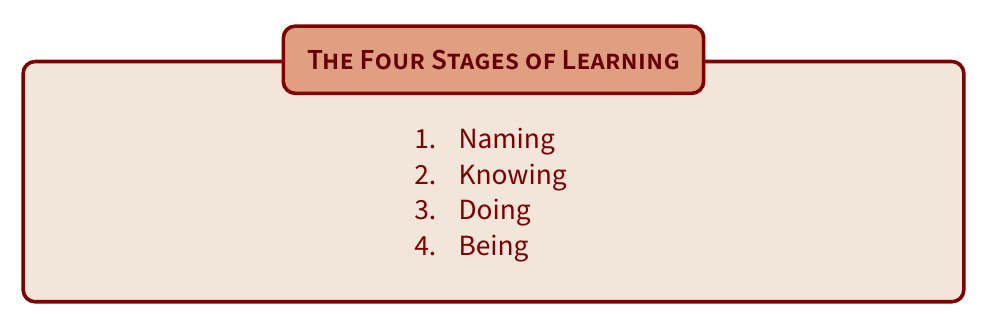
\includegraphics[width=0.9\linewidth,height=\textheight,keepaspectratio]{images/four-stages-of-learning.png}
\caption{Learning any subject involves four stages as shown above
{[}\citeproc{ref-sas}{1}{]}.}\label{fig:four-stages}
\end{figure}

All knowledge begins with \emph{naming}. You cannot analyze or
understand what you cannot name. In specialized subject areas, names are
called \emph{definitions}. In this blog, we have the following
\emph{three} mathematical names to define, understand, analyze, and
apply:

\begin{enumerate}
\tightlist
\item
  expression;
\item
  equation; and
\item
  formula.
\end{enumerate}

After naming, we move to \emph{knowing}. At this stage, we
systematically study the subject that has been defined to the extent
that we are familiar with it \emph{ourselves}, without recourse to a
teacher, a textbook, or other reference material.

The third stage, \emph{doing}, involves \emph{application} of the
newfound concept that has already been defined and studied. If you were
learning to fly an aircraft, you could not claim to be a pilot, based on
mere theoretical knowledge. You must practise flying---first under
supervision, and later solo---so that you accumulate enough experience
to claim competence in that art.

Once the doing stage has been mastered, it becomes effortless: this is
the \emph{being} stage of knowledge. You are now a master at what you
started out to learn, and can start teaching others.

Every subject of study---whether academic like mathematics, or practical
like surgery---involves these four steps and their mastery. By steadily
moving from one stage to another---finally graduating to the being
stage---you achieve mastery of your subject.

This blog is mainly concerned with the naming stage, but our discussion
will not be complete without a modicum of knowing and doing as well. Let
us begin.

\subsection{Expressions}\label{expressions}

The word
\href{https://www.etymonline.com/search?q=expression}{expression}
literally means ``(something) that is pressed out''. In the context of
mathematics, an expression is a collection of numbers or symbols that
are written out or expressed. Sometimes, the expression might seem
complicated, but it might also be amenable to simplification.

Let us start with something basic:
\begin{equation}\phantomsection\label{eq:two-plus-four}{
2 + 4
}\end{equation} It is a mathematical expression for adding four to two.
But is that not \(6\)? So, is the expression \(2 + 4\) or is it \(6\)?
The \emph{expression} itself is \emph{two plus four}. Its \emph{value}
is six.

But if we know that \(2 + 4 = 6\), why can't we say that the expression
is \(6\)? We \emph{may} if we were asked to \emph{simplify} the
expression. But the expression itself remains as it was originally
written.

Let us move up a notch. Look at:
\begin{equation}\phantomsection\label{eq:sqrt5}{
\sqrt{25}
}\end{equation} What does it mean? Now you need to know the language of
mathematics. What does \(\surd\) stand for? It is a stylized letter
``r'' for the word
\href{https://en.wikipedia.org/wiki/Square_root}{radix} which stands for
the positive square root of the number inside the symbol. What number
multiplied by itself will give us \(25\)? Well, \(5 \times 5\) equals
\(25\).

But is that all? What about \((-5) \times (-5) = 25\)? That too is
correct. So, what does \(\sqrt{25}\) really stand for? It is
\emph{defined} to be the \emph{positive} square root of \(25\) which is
\(5\).

The case of \(-5\) is catered for by the expression \(-\sqrt{25}\). We
may write \(-\sqrt{25} = -5\); thus, we do not have notational
ambiguity.

\subsubsection{Simplifying an
expression}\label{simplifying-an-expression}

In school, you might have been asked to \emph{simplify an expression}.
In that case, you are being asked to produce a result that is the same
as the original expression but is simpler in form and appearance. For
example, we could write: \begin{equation}\phantomsection\label{eq:six}{
2 + 4 = 6
}\end{equation} Look! What have we done? We have produced an
\emph{equation}. The sum of the two numbers on the left hand side (LHS)
equals the single number on the right hand side (RHS).

We will consider \emph{equations} a little later, but for now, bear in
mind, that to simplify an expression, we need to find a
\emph{mathematical alias} for it that \emph{equals} the original
expression, but is simpler in form.

\subsubsection{Enter algebra}\label{enter-algebra}

After we mature a little more mathematically, we start dealing with
numbers whose values are not known. We use \emph{letters} to denote
these unknown quantities, much like we use \emph{pronouns} instead of
\emph{proper nouns} for the names of people we do not know. Let us take
a look at a potentially confusing expression:
\begin{equation}\phantomsection\label{eq:abc}{
\dfrac{\left(\dfrac{a}{b}\right)}{c}
}\end{equation} What does it mean? Can it be simplified? If so, what is
its simplified form? Does it convey any meaning? What is the purpose of
the parentheses on top?

Mathematics is a language in which ambiguity is prohibited by strictly
enforced conventions. We already saw that with the \(\surd\) sign.

Does \cref{eq:abc}\footnote{It is not an equation but an expression; my
  software did not allow that degree of customization. Please excuse
  this inaccuracy.} mean more than one thing? Not if we know our
conventions. The expression consists of a value on top, divided by a
value at the bottom. But the value at the top is itself a fraction, that
must be evaluated first because its numerator and denominator are
bracketed or enclosed in parentheses:\footnote{See
  \hyperref[bidmas]{BIDMAS} later.}
\begin{equation}\phantomsection\label{eq:a-over-b}{
\left(\dfrac{a}{b}\right)
}\end{equation} This is now divided by the value \(c\).
\href{https://swanlotus.netlify.app/blogs/the-two-most-important-numbers-zero-and-one\#the-multiplicative-inverse-in-mathbbz-mathbbq-and-mathbbr}{We
know} that \emph{dividing} by \(c\) amounts to \emph{multiplying} by
\(\dfrac{1}{c}\). The expression may therefore be simplified
so:\footnote{Refer to the chapter ``Arithmetic Revisited'' in the
  \emph{SAS} book {[}\citeproc{ref-sas}{1}{]} if you are still unclear
  about what follows.}
\begin{equation}\phantomsection\label{eq:simplified}{
\begin{aligned}
\dfrac{\left(\dfrac{a}{b}\right)}{c} &= \left(\dfrac{a}{b} \times \dfrac{1}{c}\right)\\
&= \left(\dfrac{a \times 1}{b \times c}\right)\\
&= \left(\dfrac{a}{bc}\right)
\end{aligned}
}\end{equation} Note that the horizontal line separating the numerator
and the denominator is called the \emph{vinculum} and it is long enough
to cover \emph{both} \(b\) and \(c\) in the denominator. I have inserted
parentheses on the RHS of \cref{eq:simplified} to clarify the grouping
of terms, but strictly, they are not necessary.

If we did not have access to mathematical typesetting, this fraction
would be written unambiguously as \(a/(bc)\) where the two terms in the
denominator must be grouped together by parentheses. If instead, this
was written as \(a/bc\) the expression could also be correctly read as
\((a/b) \times c = (ac)/b\) which is different from \(a/(bc)\). This is
reason enough to justify the use of parentheses or brackets in
mathematical expressions, which we take a look at next.

\subsubsection{BIDMAS}\label{bidmas}

When a mathematical expression is evaluated, we work from left to right,
respecting
\href{https://en.wikipedia.org/wiki/Order_of_operations}{operator
precedence}. This is a convention that lays down a hierarchy or protocol
about which operation is performed before which. It is often reduced to
the \href{https://www.dictionary.com/browse/mnemonic}{mnemonic}
\href{https://en.wikipedia.org/wiki/Order_of_operations\#Mnemonics}{BIDMAS}.

The initial \emph{B} stands for brackets, or parentheses. Bracketed
expressions are evaluated first. Then we evaluate \emph{I} or indices:
powers and square roots. The \emph{DMAS} stands for division,
multiplication, addition, and subtraction in that order.

This \emph{convention} ensures that everyone is
\href{https://www.gingersoftware.com/content/phrases/on-the-same-page}{on
the same page} when evaluating mathematical expressions. All will get
the same result. Ambiguity is hence exiled from the mathematical
landscape.

If you love mathematical symbols, you might wish to remember this
unpronounceable visual mnemonic instead: \[
()x^y\div\times+-
\] Choose whichever mnemonic appeals more to you.

\subsubsection{A visual metaphor for mathematical
expressions}\label{a-visual-metaphor-for-mathematical-expressions}

My preferred visual image for a mathematical expression is a tied-up
bundle of clothes:

\begin{figure}
\centering
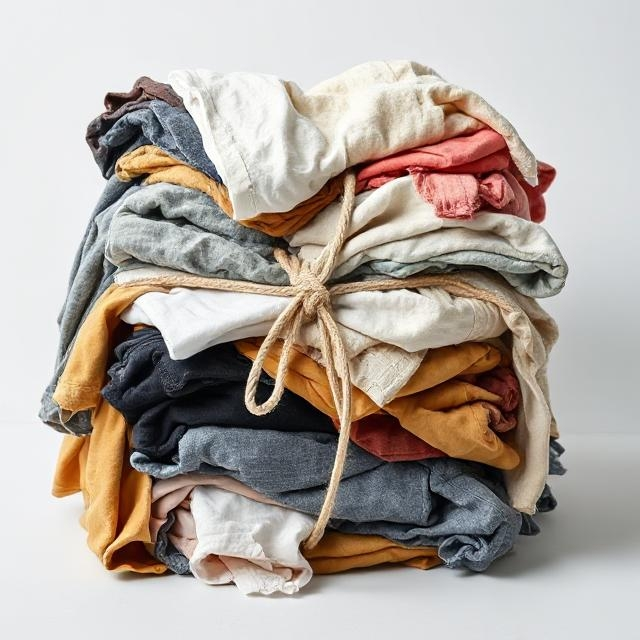
\includegraphics[width=0.8\linewidth,height=\textheight,keepaspectratio]{images/bundle-of-clothes-in-disarray.jpg}
\caption{Bundle of clothes as a visual metaphor for a mathematical
expression.}\label{fig:clothes-bundle}
\end{figure}

\subsection{Equations}\label{equations}

Let us now look at \emph{equations}. All equations embody the \(=\)
symbol, which is called an \emph{equals sign}. It is a mathematical
shorthand to denote that what is on the LHS of this symbol is equal to
what is on the RHS, however different they may appear to be. We have
previously encountered this symbol in the very simple equation \[
2 + 4 = 6.
\]

\subsubsection{Operations and relations}\label{operations-and-relations}

Before venturing further, we need to distinguish between
\emph{operations} and \emph{relations}.\footnote{I have avoided a set
  theoretic framework and notation to keep this blog within the grasp of
  young students.}

Addition, multiplication, exponentiation, etc., are familiar
\href{https://en.wikipedia.org/wiki/Binary_operation}{binary
operations}, which take two inputs or \emph{operands}, from the same
set, and produce a single output or result, again from the same set, as
in \[
2 + 4 = 6.
\]

A \href{https://en.wikipedia.org/wiki/Binary_relation}{binary relation},
on the other hand, associates elements in one set to elements in another
set via a relation \(R\). Formally, if \(x \in X\) and \(y \in Y\) and
\(R\) is a relation between the two, we denote the relation by the
\emph{ordered pair} \((x, y)\), written so: \[
xRy = (x, y)
\] whenever the relation \(R\) holds.

Equality is a binary relation in which \(R\) is replaced by the better
known \(=\) symbol. It is an
\href{https://en.wikipedia.org/wiki/Equivalence_relation}{equivalence
relation} with three properties:
\href{https://en.wikipedia.org/wiki/Reflexive_relatio}{reflexive},
\href{https://en.wikipedia.org/wiki/Symmetric_relation}{symmetric}, and
\href{https://en.wikipedia.org/wiki/Transitive_relation}{transitive}.

\begin{enumerate}
\tightlist
\item
  Reflexivity means that every number is equal to itself:
  \(2 + 4 = 2 + 4\) and \(6 = 6\).
\item
  Symmetry means that if \(2 + 4 = 6\), then \(6 = 2 + 4\). Note that
  this is \emph{not}
  \href{https://en.wikipedia.org/wiki/Commutative_property}{commutativity},
  which applies to operands, not to relations.
\item
  Transitivity means that if \(2 + 4 = 6\) and if \(6 = 3 + 3\), then
  \(2 + 4 = 3 + 3\).
\end{enumerate}

What is the need for stating these blindingly obvious properties? Were
they singled out by a bunch of people who were
\href{https://www.dictionary.com/browse/out-to-lunch}{out to lunch}? You
may be totally excused if you thought so.

But the power of these properties lies in their ability to be
generalized beyond the immediate context in which they arose: something
you would appreciate as you plumb the deeper depths and higher heights
of mathematics, with the passage of time.

In sum, a binary operation works on two inputs to produce a third
output. A binary relation, like equality, on the other hand, establishes
a relationship---sameness in this case---between two mathematical
elements.

\subsubsection{A visual metaphor for
equality}\label{a-visual-metaphor-for-equality}

A two-pan balance is an excellent visual metaphor for equality. Even
though the material in each pan might be different, when the pans
balance, we have equality. This means each pan contains the same weight
or mass. It is the principle behind how we pay for foodstuffs by weight.
And it is identical to the concept of equality as a mathematical
relation.

\begin{figure}
\centering
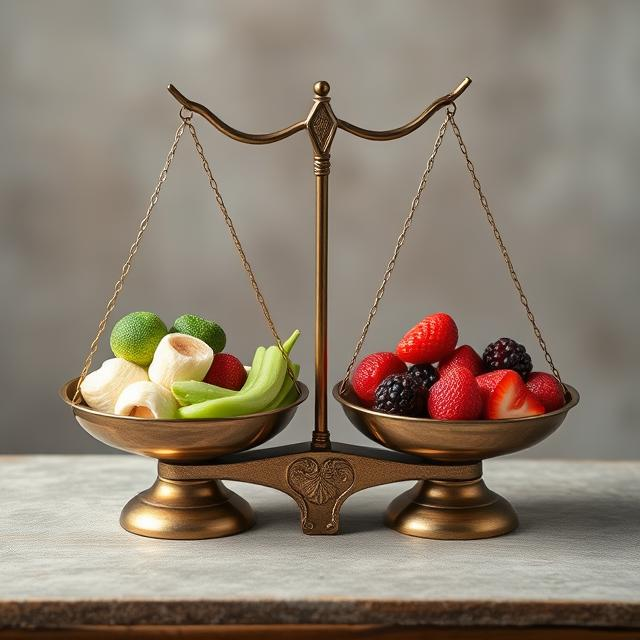
\includegraphics[width=0.9\linewidth,height=\textheight,keepaspectratio]{images/two-pan-balance-in-equilibrium.jpg}
\caption{A two-pan balance in equilibrium, indicating that the mass on
the left hand side equals that on the right hand side, even though the
contents differ.}\label{fig:two-pan-balance}
\end{figure}

\subsubsection{An example simple
equation}\label{an-example-simple-equation}

Equations demonstrate their power when used to determine unknowns. A
\emph{simple} equation has a single unknown and some statements that can
be used to \emph{solve for} the unknown. For example,

\begin{quote}
There are twice as many girls as boys in my class of thirty students.
How many are boys?
\end{quote}

Those of you who can think in numbers might have mentally solved the
problem by juggling numbers in your head: 10 boys and 20 girls.

What if you cannot do that? The power of mathematics lies in its
discovery of \emph{systematic methods} to solve all manner of problems,
regardless of the abilities of the person solving the question.

The primary skill in dealing with such \emph{word questions} is the
ability to translate the written words into mathematical expressions and
equations.

The first step is to define the variables or unknowns. What is it that
we are asked to determine? The number of boys. Let \(b\) be the number
of boys.

There are twice as many girls as boys. If \(g\) is the number of girls,
\(g = 2b\) as they are double the number of boys.

The total number of students is \(30\).

Here is the logical thread we follow: \[
\begin{aligned}
g + b &= 30; \text{ but $g = 2b$, and substituting, we get}\\
2b + b &= 30; \text{ adding}\\
3b &= 30; \text{ dividing by $3$ on both sides to get $b$}\\
b &= 10; \text{ and we are done.} 
\end{aligned}
\]

\subsubsection{The ``\ldots nomial'' family}\label{the-nomial-family}

Let us detour a little to review expressions again. Expressions that
satisfy certain conditions appear again and again, enough to warrant
being given special names. We consider here,
\href{https://en.wikipedia.org/wiki/Monomial}{monomial},
\href{https://en.wikipedia.org/wiki/Binomial_(polynomial)}{binomial},
\href{https://en.wikipedia.org/wiki/Trinomial}{trinomial}, and
\href{https://en.wikipedia.org/wiki/Polynomial}{polynomial}.

A monomial is defined as a constant, a variable, or a product of
variables, each raised to a non-negative integer exponent. It is an
expression consisting of just \emph{a single term}.

A binomial is the sum of two monomials. A trinomial is the sum of three
monomials. And, finally, a polynomial is the sum of three or more
monomials. Note that
\href{https://swanlotus.netlify.app/blogs/the-two-most-important-numbers-zero-and-one}{by
sum, we also include subtraction}.

A single number by itself like \(42\) or \(-17\) is a (constant)
monomial. When the number appears as part of a variable, like \(42x^2\),
the \(42\) is called the \emph{coefficient} of the variable \(x^2\).
Note that
\href{https://swanlotus.netlify.app/blogs/the-two-most-important-numbers-zero-and-one}{a
standalone constant may also be viewed as the coefficient of a variable
raised to the zeroth power}, e.g, \(42 = 42x^{0}\). In this blog, we
deal only with real coefficients.

\begin{longtable}[]{@{}
  >{\raggedright\arraybackslash}p{(\linewidth - 6\tabcolsep) * \real{0.1765}}
  >{\raggedright\arraybackslash}p{(\linewidth - 6\tabcolsep) * \real{0.1912}}
  >{\raggedright\arraybackslash}p{(\linewidth - 6\tabcolsep) * \real{0.3235}}
  >{\raggedright\arraybackslash}p{(\linewidth - 6\tabcolsep) * \real{0.3088}}@{}}
\caption{\label{tbl:nomials}Monomials, binomials, trinomials, and
polynomials}\tabularnewline
\toprule\noalign{}
\begin{minipage}[b]{\linewidth}\raggedright
Name
\end{minipage} & \begin{minipage}[b]{\linewidth}\raggedright
Prefix
\end{minipage} & \begin{minipage}[b]{\linewidth}\raggedright
Meaning
\end{minipage} & \begin{minipage}[b]{\linewidth}\raggedright
Examples
\end{minipage} \\
\midrule\noalign{}
\endfirsthead
\toprule\noalign{}
\begin{minipage}[b]{\linewidth}\raggedright
Name
\end{minipage} & \begin{minipage}[b]{\linewidth}\raggedright
Prefix
\end{minipage} & \begin{minipage}[b]{\linewidth}\raggedright
Meaning
\end{minipage} & \begin{minipage}[b]{\linewidth}\raggedright
Examples
\end{minipage} \\
\midrule\noalign{}
\endhead
\bottomrule\noalign{}
\endlastfoot
Monomial & mono & one term & \(12, a, cx^2, \frac{b}{3}, -97, xyz\) \\
Binomial & bi & two terms & \(a - b, 3r^4 - pq, \frac{1}{5}x + uvw\) \\
Trinomial & tri & three terms & \(x^2 - 2x + 1, u + v + w\) \\
Polynomial & poly & many terms & \(25x^3 + 4y^2 + z^4 + 37\) \\
\end{longtable}

What sort of terms do \emph{not} qualify to be one of the ``nomials''?
What about \(c^{\frac{1}{5}}\)? A fractional power like \(\frac{1}{5}\)
is not an integer, let alone a non-negative integer. So, it does not
qualify. Consider also \(x^{-5}\). No again, as \(-5\) is a negative
integer.

\subsubsection{Quadratics}\label{quadratics}

Thus far we have encountered \emph{linear} equations, in which the
highest power of the variable is \(1\), and the other terms are
constants. But just as numbers can be multiplied, so too can expressions
containing variables. Consider:
\begin{equation}\phantomsection\label{eq:quad-expand}{
\begin{aligned}
(x - 5)^{2} &= (x - 5)(x - 5); \text{ multiplying the two terms}\\
&= x^2 +x(-5) + (-5)x + (-5)(-5)\\
&= x^2 - 10x + 25
\end{aligned}
}\end{equation} The expression on the left is a binomial multiplied by
another binomial and the product is a trinomial. But this product is
also called a \href{https://en.wikipedia.org/wiki/Quadratic}{quadratic
polynomial}, because it is a square. Indeed any expression in one
variable in which the highest power of the variable is \(2\) qualifies
as a quadratic.\footnote{You don't need this here, but just for
  completeness, if there are more than one variable and all terms are of
  degree \(2\), e.g., \(x^2 + xy + y^2\), the expression is called a
  \href{https://en.wikipedia.org/wiki/Quadratic_form}{quadratic form}.}
Be aware that the same expression could be called by different names
depending upon the context in which it is viewed.

When a quadratic polynomial is equated to zero, we have a
\href{https://en.wikipedia.org/wiki/Quadratic_equation}{quadratic
equation}. Let us convert the quadratic in \cref{eq:quad-expand} into
the quadratic equation
\begin{equation}\phantomsection\label{eq:repeated-root}{
\begin{aligned}
x^2 -10x + 25 &= 0\\
(x - 5)^2 &= 0\\
(x - 5)(x - 5) &= 0\\
x &= 5.
\end{aligned}
}\end{equation} This is a case of a quadratic that is a perfect square
and the root \(x = 5\) is \emph{repeated}.

We may graph the
\href{https://en.wikipedia.org/wiki/Quadratic_function}{quadratic
function}, \(y = x^2 -10x + 25\), on \(x\)-\(y\) coordinate axes as
shown in \cref{fig:quadratic-graphs}. The solution(s) to the quadratic
equation \(x^2 -10x + 25 = 0\) then occur when \(y = 0\). But the upper
curve intersects the \(x\)-axis at only one point, i.e., it is
\emph{tangent} to the \(x\)-axis. So, the root \(x = 5\) is
\emph{repeated}.

But what happens when the root is not repeated? Let us look at
\(x^2 - 25 = 0\), which is a
\href{https://en.wikipedia.org/wiki/Difference_of_two_squares}{difference
of two squares}:
\begin{equation}\phantomsection\label{eq:plus-minus-five}{
\begin{aligned}
x^2 - 25 &= 0;\\
x^2 -5^2 &= 0;\\
(x + 5)(x - 5) &= 0;\\
x &= -5 \text{ or} +5.\\ 
\end{aligned}
}\end{equation} In this case we have two \emph{distinct} roots:
\(x = \pm5\). Again, see \cref{fig:quadratic-graphs} where the lower
curve intersects the \(x\)-axis, or \(y=0\) line, at these two distinct
points.

\begin{figure}
\centering
\includesvg[width=0.8\linewidth,height=\textheight,keepaspectratio]{images/quadratic.svg}
\caption{Graphs of the two quadratic equations discussed in the text.
The solutions to the respective quadratic equations are the values of
\(x\) at which the curves intersect the
\(x\)-axis.}\label{fig:quadratic-graphs}
\end{figure}

\subsubsection{Completing the square and the quadratic
formula}\label{completing-the-square-and-the-quadratic-formula}

Around the ninth or tenth year of middle school, you would have been
exposed to the
\href{https://en.wikipedia.org/wiki/Quadratic_formula}{quadratic
formula} for computing the roots of a quadratic equation, without
recourse to factorization or graphing, as we have done above.

Let us derive the quadratic formula by a method known as
\href{https://en.wikipedia.org/wiki/Completing_the_square}{``completing
the square''}. The generic quadratic equation is
\begin{equation}\phantomsection\label{eq:orig-quad}{
ax^2 + bx + c = 0.
}\end{equation} By applying the same operations to both sides, we
manipulate \cref{eq:orig-quad} to resemble, term by term, a perfect
square, and then extract the root without fuss. Here are the steps in
the algorithm:

\begin{enumerate}
\item
  Divide through \cref{eq:orig-quad} by \(a\) to make the coefficient of
  \(x^2\) one. Because zero divided by any non-zero number is still
  zero, we have \begin{equation}\phantomsection\label{eq:no-a}{
  \frac{a}{a}x^2 + \frac{b}{a}x + \frac{c}{a} = x^2 + \frac{b}{a}x + \frac{c}{a} = 0.
  }\end{equation} Let \cref{eq:no-a} be called the \emph{normalized}
  quadratic equation.
\item
  Let us digress a little. Consider a linear binomial term in \(x\),
  like \((x + k)\), with \(k\) being a real constant, and square it.
  Then, \((x + k)^2 = x^2 + 2kx + k^2\) for all \(x\) and
  \(k\).\footnote{This is an \hyperref[identities]{identity}.} The
  middle term, containing \(x\), \emph{always} has a factor of \(2\) in
  it.
\item
  To insert an explicit factor of \(2\) in the term for \(x\), in the
  normalized quadratic equation, we divide the term containing \(x\) by
  \(2\) and then multiply it by \(2\), preserving the rest of the
  coefficient, thus: \[
  \left(\frac{b}{a}\right)x = 2\left(\frac{b}{2a}\right)x.
  \]
\item
  The equation now becomes
  \begin{equation}\phantomsection\label{eq:normalized-one}{
  x^2 + 2\left(\frac{b}{2a}\right)x + \frac{c}{a} = 0.
  }\end{equation}
\item
  Observe that \begin{equation}\phantomsection\label{eq:extra-term}{
  \begin{aligned}
  \left(x + \frac{b}{2a}\right)^2 &= x^2 + 2\left(\frac{b}{2a}\right)x + \left(\frac{b}{2a}\right)^2\\
  &= x^2 + 2\left(\frac{b}{2a}\right)x + \left(\frac{b^2}{4a^2}\right).
  \end{aligned}
  }\end{equation}
\item
  Note that when \cref{eq:extra-term} is compared to
  \cref{eq:normalized-one}, the constant term
  \(\left(\dfrac{b^2}{4a^2}\right)\) has now been inserted extraneously
  by virtue of our simulating a square. It must be removed by
  subtraction to restore the original \cref{eq:normalized-one}, so that
  our equation becomes:
  \begin{equation}\phantomsection\label{eq:quad-formula}{
  \begin{aligned}
  \left(x + \frac{b}{2a}\right)^2 - \left(\frac{b^2}{4a^2}\right) + \frac{c}{a} &= 0; \text{ leading to}\\
  \left(x + \frac{b}{2a}\right)^2 &= \left(\frac{b^2}{4a^2}\right) - \frac{c}{a}\\
  &= \frac{b^2}{4a^2} - \frac{4ac}{4a^2}\\
  &= \frac{b^2 - 4ac}{4a^2}; \text{ take square roots on both sides}\\
  \left(x + \frac{b}{2a}\right) &= \pm\sqrt{\frac{b^2 - 4ac}{4a^2}}; \text{ transpose $\frac{b}{2a}$ from left to right}\\
  x &= -\frac{b}{2a} \pm \frac{\sqrt{b^2 - 4ac}}{2a}\\
  &=\frac{-{b} \pm \sqrt{b^2 - 4ac}}{2a}
  \end{aligned}
  }\end{equation} Some of you might have found it hard to keep up with
  the symbolic jugglery to arrive at the final form of
  \cref{eq:quad-formula}, and I sympathize with you.
\end{enumerate}

But there is a geometric side to most mathematical problems. So, if
pictures appeal more to you, I suggest watching a YouTube video or three
to better understand the dance of the symbols above. I recommend these
three videos to help clarify the motivation and geometric basis for the
quadratic formula, arrived at by completing the square:

\begin{enumerate}
\def\labelenumi{\alph{enumi}.}
\item
  \href{https://www.youtube.com/watch?v=T0HyWIFbsHQ}{Completing the
  Square (visual proof)} {[}\citeproc{ref-mvp-2022}{2}{]};
\item
  \href{https://www.youtube.com/watch?v=7Q4h1YTYgnE}{But where does the
  quadratic formula come from?}
  {[}\citeproc{ref-foggy-maths-2023}{3}{]}; and
\item
  \href{https://www.youtube.com/watch?v=McDdEw_Fb5E}{Beautiful Visual
  Explanation of Completing the Square}
  {[}\citeproc{ref-woo-2016}{4}{]}.
\end{enumerate}

I am confident that at least one of these explanations will resonate
with you, and that you will get a
\href{https://nesslabs.com/eureka-moments}{eureka moment} once the
method clicks. It is only then that you have made some of this knowledge
your own through self-effort.

As always, there is more to the quadratic formula than has been
discussed here. The value of the expression under the square root,
\((b^2 - 4ac)\), called the
\href{https://www.britannica.com/science/discriminant}{discriminant},
helps determine the \emph{nature} of the roots of the quadratic
equation, without actually having to solve the equation:

\begin{enumerate}
\def\labelenumi{\alph{enumi}.}
\item
  If the discriminant is positive, the roots will be real and distinct;
\item
  If the discriminant is zero, there will be a real, repeated root;
\item
  If the discriminant is negative, the roots will be a
  \href{https://www.mathcentre.ac.uk/resources/sigma\%20complex\%20number\%20leaflets/sigma-complex6-2009-1.pdf}{complex
  conjugate} pair.
\end{enumerate}

There are other interesting properties as well, but I will stop here.

\subsubsection{Identities}\label{identities}

A mathematical
\href{https://en.wikipedia.org/wiki/Identity_(mathematics)}{identity} is
an equation or equality which is true regardless of the values assumed
by the variables in it. The two sides of an identity are usually quite
different in appearance, and it is this difference that confers on them
their importance and usefulness.

Simply by expanding and multiplying out, we know that \[
(a+b)^2 = a^2 +2ab + b^2. 
\] To stress that this is no ordinary equation but an identity, it may
also be written as \[
(a+b)^2 \equiv a^2 +2ab + b^2.
\] The three-line symbol is called a
\href{https://en.wikipedia.org/wiki/Triple_bar}{triple bar}, although
the the more youthful among us might recognize it as the
\href{https://en.wikipedia.org/wiki/Hamburger_button}{hamburger symbol}.

Identities arise in different contexts and the Pythagorean theorem,
applied to the unit circle, gives rise to the well known trigonometric
identity \[
\cos^2\theta + \sin^2\theta \equiv 1.
\]

\subsection{Formulae}\label{formulae}

Formulae arise in different contexts. Water when expressed chemically is
H\textsubscript{\(2\)}O. The word
\href{https://www.vocabulary.com/dictionary/formulation}{formulation}
refers to a collection of ingredients prepared according to a specific
recipe to serve a specific purpose. An ancient
\href{https://pmc.ncbi.nlm.nih.gov/articles/PMC6571565/\#:~:text=Chyawanprash\%20is\%20formulated\%20by\%20processing,richest\%20source\%20of\%20vitamin\%20C}{vitality
enhancing tonic}, for example, consists of dozens of ingredients
combined in a specified way.

But the \href{https://en.wikipedia.org/wiki/Formula}{formulae} we refer
to here are succinct mathematical statements whose truth has been
established, and whose use saves time and effort. In this sense, all
\href{https://en.wikipedia.org/wiki/Formula}{theorems} are formulae.
They save us having to re-invent the wheel each time we are faced with
an already-solved task.

Early encounters with mathematical formulae arise with simple equations
for the area of a triangle (A = \(\frac{1}{2}bh\)), the circumference of
a circle (\(C = 2\pi r\)), or the volume of a sphere
(\(V = \frac{4}{3}\pi r^3\)).

The importance of formulae as conveniences is summarized by this
quotation from the famous computer scientist
\href{https://en.wikipedia.org/wiki/Edsger_W._Dijkstra}{Edsger Dijkstra}
{[}\citeproc{ref-dijkstra-hand}{5},\citeproc{ref-dijkstra-html}{6}{]}\footnote{I
  highly recommend readers of this blog to read Professor Dijkstra's
  exemplary essay. It exhibits the elegance characteristic of a rounded
  scholar of yesteryear, who is knowledgeable not only in mathematics
  and logic, but also in Latin, history, and philosophy.} :

\begin{quote}
``A picture may be worth a thousand words, a formula is worth a thousand
pictures.''
\end{quote}

And with that memorable quote, I conclude this blog, lest it stretch to
infinity!

\subsection{Acknowledgements}\label{acknowledgements}

I acknowledge the valuable contributions from several readers of my blog
who shall remain anonymous. Their insights, carrying the fresh
viewpoints of students, helped to clarify much that was still unclear.

\subsection{Feedback}\label{feedback}

Please \href{mailto:feedback.swanlotus@gmail.com}{email me} your
comments and corrections.

\noindent A PDF version of this article is
\href{./expressions-equations-formulae.pdf}{available for download
here}:

\begin{small}

\begin{sffamily}

\url{https://swanlotus.netlify.app/blogs/expressions-equations-formulae.pdf}

\end{sffamily}

\end{small}

\section*{References}\label{bibliography}
\addcontentsline{toc}{section}{References}

\phantomsection\label{refs}
\begin{CSLReferences}{0}{0}
\bibitem[\citeproctext]{ref-sas}
\CSLLeftMargin{{[}1{]} }%
\CSLRightInline{R (Chandra) Chandrasekhar. 2025. {Secrets of Academic
Success}: {Timeless Principles for Lifelong Learning}. Retrieved 11
February 2025 from
\url{https://swanlotus.netlify.app/sas-manuscript/SAS-partial.pdf}}

\bibitem[\citeproctext]{ref-mvp-2022}
\CSLLeftMargin{{[}2{]} }%
\CSLRightInline{Mathematical Visual Proofs. 2022. {Completing the Square
(visual proof)}. Retrieved 15 February 2025 from
\url{https://www.youtube.com/watch?v=T0HyWIFbsHQ}}

\bibitem[\citeproctext]{ref-foggy-maths-2023}
\CSLLeftMargin{{[}3{]} }%
\CSLRightInline{FoggyMaths. 2023. {But where does the quadratic formula
come from?} Retrieved 15 February 2025 from
\url{https://www.youtube.com/watch?v=7Q4h1YTYgnE}}

\bibitem[\citeproctext]{ref-woo-2016}
\CSLLeftMargin{{[}4{]} }%
\CSLRightInline{Eddie Woo. 2016.{ Beautiful Visual Explanation of
Completing the Square}. Retrieved 15 February 2025 from
\url{https://www.youtube.com/watch?v=McDdEw_Fb5E}}

\bibitem[\citeproctext]{ref-dijkstra-hand}
\CSLLeftMargin{{[}5{]} }%
\CSLRightInline{Edsger W.Dijkstra. 1996. {A first exploration of
effective reasoning}. {Handwritten manuscript, University of Texas at
Austin}. Retrieved 14 February 2025 from
\url{https://www.cs.utexas.edu/~EWD/ewd12xx/EWD1239.PDF}}

\bibitem[\citeproctext]{ref-dijkstra-html}
\CSLLeftMargin{{[}6{]} }%
\CSLRightInline{Edsger W.Dijkstra. 1996. {A first exploration of
effective reasoning}. {HTML transcript, University of Texas at Austin}.
Retrieved 14 February 2025 from
\url{https://www.cs.utexas.edu/~EWD/transcriptions/EWD12xx/EWD1239.html}}

\end{CSLReferences}



\end{document}
